\section{An authority-preserving delayed term}\label{sec:delayed}

Under DVF the forced orbit takes most of the command. At \SI{2500}{\rpm} with $g=\SI{1500}{\volt\second\per\metre}$, $\bmax$ is 6.2--\SI{8.6}{\volt} at 18 of the 34 depths below $\alim$ on a \SI{0.5}{\milli\metre} grid, and it falls to \SI{0.17}{\volt} only near the axial pitch, where the helix cancels the tooth harmonics [Eq.~\eqref{eq:Fm}]. The level $u_0$ of the sector condition~\eqref{eq:sector}, which sets the certified basin (Section~\ref{sec:certificates}), is then only 0.4--\SI{2.8}{\volt}. This section asks whether the authority can be spent on the deviation from the orbit alone.
% src: results/c4_limits.npz (2500 rpm, g = 1500: bmax on the 0.5 mm depth grid; 18 of the 34 depths below a_lim = 17.24 mm at 6.20-8.57 V, i.e. u0 = 0.43-2.80 V; minimum 0.17 V at 12.5 mm); README §13.1

\subsection{The law and its properties}\label{sec:delayed-law}

The DVF command of Eq.~\eqref{eq:dvf} is replaced by
\begin{equation}\label{eq:comb-law}
  u(t)=-g_1\dot x(t)-g_2\bigl[\dot x(t)-\dot x(t-T)\bigr]-k_d\bigl[x(t)-x(t-T)\bigr],
\end{equation}
and clipped as before, $V=\sat_{\Vmax}(u)$. This is DVF plus a proportional--derivative feedback of the displacement difference over one tooth period; designs with $k_d=0$ are denoted DVF\,+\,D and designs with $g_2=0$ DVF\,+\,P. In the Laplace domain $U(s)=-\bigl[s\,K(s)+k_d\,E(s)\bigr]X(s)$, with the scalar transfer functions (not the row $K$ and the matrix $E$ of Eq.~\eqref{eq:coll})
\begin{equation}\label{eq:comb-K}
  K(s)=g_1+g_2\,E(s),\qquad E(s)=1-e^{-sT}.
\end{equation}

\emph{(i)~The delayed terms vanish on the forced orbit.} $E$ is a comb filter with a zero at every tooth-passing harmonic, $E(im\omega_T)=1-e^{-i2\pi m}=0$; equivalently, $x(t)=x(t-T)$ on any $T$-periodic motion. The forced orbit is therefore the DVF orbit of Eq.~\eqref{eq:xp} with $g=g_1$, and its command is $b(t)=-g_1\dot x_p(t)$ for any $g_2$ and $k_d$: the forced command, $\bmax$ and $u_0$ depend on $g_1$ alone, while a deviation from the orbit meets the full law.

\emph{(ii)~DVF\,+\,D is passive only without loop delay.} The P term is not passive: the real part of $k_dE(i\omega)/(i\omega)$, $k_d\sin(\omega T)/\omega$, changes sign. For $g_1,g_2\ge0$ and $\operatorname{Re}s\ge0$, $\operatorname{Re}K(s)=g_1+g_2\bigl[1-e^{-T\operatorname{Re}s}\cos(T\operatorname{Im}s)\bigr]\ge g_1$: $K$ is positive real, and with an ideal collocated force actuator and an instantaneous loop the velocity loop is passive, like DVF \citep{elliott2001feedback}. A loop delay $\tau$ (not the segment length $\tau=T/M$ of Section~\ref{sec:cert-periodic}) makes the controller $e^{-s\tau}K(s)$, and the phase of $E(i\omega)$, which sweeps from $+\ang{90}$ to $-\ang{90}$ between consecutive tooth-passing harmonics, adds to the lag of the delay in the upper half of each interval, where it is negative (Section~\ref{sec:delayed-robust}). $\lvert K(i\omega)\rvert$ ranges from $g_1$ at the harmonics to $g_1+2g_2$ halfway between them.

\emph{(iii)~$k_d$ must be negative.} The mean regenerative force $\overline{aH}\,[x-x(t-T)]$ has $\overline{aH}<0$ [Eq.~\eqref{eq:aHmean}], so $k_d<0$ opposes it and $k_d>0$ reinforces it. As $G_a\approx K_a$ at the chatter frequency, each $-\SI{e5}{\volt\per\metre}$ of $k_d$ contributes $K_a\times\SI{e5}{\volt\per\metre}=\SI{3e5}{\newton\per\metre}$ to the coefficient of $x-x(t-T)$, which is the magnitude $N_tK_{tc}\lvert\alpha_{yy}\rvert a/(4\pi)$ of the mean regenerative coefficient at $a=\SI{1}{\milli\metre}$, and so offsets about \SI{1}{\milli\metre} (\SI{0.98}{\milli\metre} at \SI{2500}{\rpm}, $g_1=1500$).
% src: README §13.2; src/c4_comb.py (docstring, model), src/c4_robust.py (controller); tests/test_c4_comb.py (test_comb_terms_vanish_on_the_settled_cut; test_negative_kd_opposes_regeneration: +0.98 mm for kd = -1e5 V/m at 2500 rpm, g1 = 1500); N_t K_tc |alpha_yy|/(4 pi) x 1 mm = 3.0008e5 N/m from src/params.py; |G_a|/K_a = 1.004 at 129.3 Hz (Section 2.1)

\subsection{Prior work and what is added}\label{sec:delayed-prior}

The law is published. Its non-invasiveness on the periodic orbit is that of Pyragas-type delayed feedback \citep{pyragas1992continuous}, which \citet{vandewouw2015ifac} and \citet{vandijk2015ijrnc} applied to high-speed milling, the latter with fixed-structure delayed output feedback that vanishes on the periodic solution and with the actuator forces as a design criterion. \citet{li2022ijamt} fed back $x(t)-x(t-T)$ through a PD law to lower the actuator voltage, delayed feedback has countered the regenerative effect in turning \citep{mancisidor2019mechatronics} and milling \citep{du2022time}, and \citet{du2024ijms} combined it with robust control and reported control voltages 11--\SI{25}{\percent} below those of robust control alone, the same authority argument. What is added here is the analysis under a hard \SI{9}{\volt} clip: the authority budget left by the forced orbit, the certified basin with the delayed terms in the sector argument (Section~\ref{sec:cert-lmi}), the gains that maximise it, their check in the simulator, and the robustness limits of the idealised model.
% src: README §13.2 (prior work; 11-25 % for Du et al. 2024); paper/notes/novelty.md §1.6 (descriptions from abstracts; the full text of vandewouw2015ifac was not checked)

\subsection{Models, certificate and simulator}\label{sec:delayed-model}

\paragraph{Certificate}
The collocated model~\eqref{eq:coll} keeps its form, with the DVF row $K=-g\,e_2^\top$ replaced by
\begin{equation*}
  \begin{gathered}
    K=-(g_1+g_2)\,e_2^\top+g_2\,d_N^\top-k_d\,\bigl(e_1-e_{4+N}\bigr)^\top,\\
    d_N^\top\xi=\frac2T\Bigl[D_{N0}\,\tilde x+\sum_{l=1}^{N}D_{Nl}\,\tilde x(t+\vartheta_l)\Bigr],
  \end{gathered}
\end{equation*}
where $e_{4+N}^\top\xi=\tilde x(t-T)$ and $d_N^\top\xi$, the derivative of the Chebyshev interpolant of the history at $\vartheta=-T$ (\ref{app:lmi}), stands for $\dot{\tilde x}(t-T)$. Since $b(t)$ depends on $g_1$ only, the orbit, $\bmax$ and the sector condition~\eqref{eq:sector} are unchanged, and the LMIs \eqref{eq:lmi-dec}--\eqref{eq:lmi-size} and the check of Section~\ref{sec:cert-check} apply as they stand. A velocity kick, however, leaves a kink in the history that the interpolant smooths: the delayed command of the model then departs from that of the delay equation by about half of $g_2\Delta v$ in each of the first two tooth periods after a kick $\Delta v$, against less than \SI{1}{\percent} of $g\Delta v$ for DVF. The certificate therefore rests more on the simulator check (Section~\ref{sec:delayed-valid}) than those of Section~\ref{sec:certificates} do.
% src: src/c4_comb.py (model, certify_kick; docstring: 0.45-0.5 and 0.5-0.65 g2 per m/s of kick); tests/test_c4_comb.py (test_comb_model_without_comb_is_the_c2_model, test_comb_row_vanishes_on_a_tooth_periodic_state, test_comb_limit_converges_in_the_nodes: limit moves < 1e-4 with 1.6x and 2.4x the nodes at 2500 rpm); README §13.3

\paragraph{Simulator}
A second build of the simulator of \ref{app:simulator}, used only when a new option is requested, adds: $g_2$ and $k_d$, with $\dot x(t-T)$ from the derivative of the cubic Hermite interpolant of the stored history (zero before $t=0$); a comb delay $T_c=\rho T$ in place of $T$ in Eq.~\eqref{eq:comb-law}, for a speed error ($\rho\approx1$) or a spindle-period comb ($\rho=N_t$); an eccentric radial runout $r_j=r_0\cos(2\pi j/N_t+\theta_r)$ of tooth $j$, which adds $r_j-r_{j+k}$ (indices modulo $N_t$) to the chip cut against the pass $k$ tooth periods back; and a loop delay $\tau$. The default build is bit-identical to that of Sections~\ref{sec:feasibility}--\ref{sec:certificates}.
% src: README §13.3 (identical preprocessed source and disassembly, fingerprint test); src/tdsim.c (COMB build), src/c4_robust.py (runout model); tests/test_c4_comb.py (test_comb_build_with_vanishing_gains_is_the_default, test_delayed_velocity_of_the_comb_term, test_loop_delay_uses_the_motion_one_delay_back, test_spindle_comb_vanishes_on_the_runout_orbit)

\paragraph{Closed form}
The robustness study uses the averaged model in the frequency domain, with the characteristic function
\begin{equation}\label{eq:comb-char}
  \begin{aligned}
    \Delta(s)&=1-G(s)\Bigl[\overline{aH}\,E(s)-G_a(s)\,e^{-s\tau}\bigl(s\,[g_1+g_2E_c(s)]+k_d\,E_c(s)\bigr)\Bigr],\\
    E_c(s)&=1-e^{-sT_c},
  \end{aligned}
\end{equation}
where $G$ may include an assumed second mode at the same point; with $\tau=0$, $T_c=T$ and one mode, $\Delta=0$ is the characteristic equation of the averaged delay equation that the collocated model approximates. Zeros in $\operatorname{Re}s>0$ were counted by the argument principle along the imaginary axis up to \SI{5}{\kilo\hertz}. The forced orbit, spindle-periodic with runout, has the harmonics $X_k=G(ik\Omega)F_k/\Delta(ik\Omega)$, with $F_k$ from the static force of one slice over a revolution, integrated over the depth as in Eq.~\eqref{eq:Fm} with $mN_t$ replaced by $k$ (without runout, $F_{mN_t}=F_m$). The closed-form limits agree with the collocated ones within $2\times10^{-4}$, and the simulated limits are 1.003--1.015 times the closed-form ones in seven cases that include the spindle comb, comb-delay errors of $\pm\SI{2}{\percent}$ and loop delays of 200--\SI{400}{\micro\second}. The settled command agrees within \SI{1.3}{\percent} in seven of eight cases with runout or delay errors, and differs by \SI{0.22}{\volt} in the eighth, where it is only about \SI{1}{\volt}.
% src: src/c4_robust.py (delta, unstable_zeros: W_MAX = 2 pi x 5 kHz, DW = 0.25 rad/s; slice_force_revolution, orbit_command); tests/test_c4_comb.py (test_closed_form_limit_is_the_collocated_limit, 4 cases, rel 2e-4; test_comb_limit_matches_the_simulator, 3 cases, rel 1.5 %); results/c4_robust.npz (td_limit ratios 1.0025-1.0148, 7 cases; td_orbit ratios 0.990-1.013 in 7 cases; 0.988 V against 0.767 V, i.e. 29 %, at 1090 rpm, 25 mm, spindle comb, 3 um runout); README §13.3

\subsection{A fair baseline and the linear limit}\label{sec:delayed-limit}

The bound $g\le\SI{1500}{\volt\second\per\metre}$ of Sections~\ref{sec:feasibility}--\ref{sec:certificates} is a choice of this study, not a property of the actuator, and a comparison at that bound inflates the benefit: added to those gains, $g_2=\SI{2000}{\volt\second\per\metre}$ doubles the linear limit (median ratio 2.00). Both families were therefore designed by the rule of Eq.~\eqref{eq:feas}: $g_1$ is the largest gain up to \SI{3000}{\volt\second\per\metre} whose steady forced command stays within \SI{9}{\volt} at every depth up to 0.9 times the design's own limit, the first unstable depth of the collocated model (found by an upward scan and bisection, as stability need not be monotone in the depth). For DVF this is the map with $g_{\max}=3000$ of Section~\ref{sec:feas-res}: the gain is limited by authority at 195 of the 251 speeds (\SIrange{1060}{3000}{\rpm}) and by the bound at the other 56. Adding $g_2$ or $k_d$ changes $g_1$ by at most \SI{10}{\volt\second\per\metre} (Fig.~\ref{fig:dlim}c), because the forced demand peaks below $0.9\alim$ of either design; in effect, the same gain is compared with and without the delayed term.
% src: results/c4_limits.npz (a_lim at the C1/C2 gain + g2 = 2000: median ratio 2.005; feas_g1: DVF below 3000 at 195 speeds, 1060-3000 rpm; max |g1 - g1_DVF| = 9.7 V s/m, 0.35 %); results/c4_summary.json (limits); src/c4_comb.py (a_lim_ctrl, feasible_g1); tests/test_c4_comb.py (test_feasible_dvf_gain_is_the_feasibility_optimum); README §13.4

With $g_2=2000$ the limit rises by a median factor of 1.78 (1.44--2.10; Table~\ref{tab:dlim}, Fig.~\ref{fig:dlim}a), and by 1.43 and 2.40 with $g_2=1000$ and 4000. The rise is largest where DVF is limited by authority, but it persists where DVF sits on the bound. As the bound applies to $g_1$ while $\lvert K\rvert$ peaks at $g_1+2g_2$, it was lifted to \SI{20000}{\volt\second\per\metre} for both families at those 56 speeds: the DVF gain then rises to \SIrange{3008}{8761}{\volt\second\per\metre}, and DVF\,+\,D ($g_2=2000$) still reaches 1.31--1.68 times the DVF limit (median 1.47). The D term thus adds linear margin at no cost on the orbit, which is more than a redistribution of authority. The P term shifts the limit by a nearly constant 2.9--\SI{3.0}{\milli\metre} ($k_d=-\SI{3e5}{\volt\per\metre}$) or 9.7--\SI{9.9}{\milli\metre} ($-\SI{e6}{\volt\per\metre}$) at every speed, as (iii) predicts.
% src: results/c4_summary.json (limits.feasible; limits.uncapped: 56 speeds, DVF g1 3008-8761 V s/m, d2000/DVF 1.31-1.68, median 1.47); results/c4_limits.npz (feas_a_lim differences, recomputed: p3e5 - dvf 2.89-3.02 mm, p1e6 - dvf 9.66-9.93 mm); README §13.4, §13.5

\begin{table}[!tbp]
  \centering
  \caption{Linear stability limit over 251 speeds (\SIrange{500}{3000}{\rpm}) under the same authority rule [Eq.~\eqref{eq:feas} with the design's own $\alim$, $g_1\le\SI{3000}{\volt\second\per\metre}$]; $g_2$ in \si{\volt\second\per\metre}, $k_d$ in \si{\volt\per\metre}. Ratio to the DVF limit at the same speed: median (range) over all speeds; last column: median over the 195 speeds where the DVF gain is limited by authority / over the 56 where it sits on the bound.}
  \label{tab:dlim}
  \small
  \begin{tabular}{@{}lccc@{}}
    \toprule
    Design & $\alim$ (\si{\milli\metre}) & Ratio to DVF & Median ratio\\
     & & median (range) & authority / bound\\
    \midrule
    DVF & 13.96--42.75 & 1 & --\\
    DVF\,+\,D, $g_2=1000$ & 21.85--54.26 & 1.43 (1.23--1.57) & 1.43 / 1.34\\
    DVF\,+\,D, $g_2=2000$ & 29.18--64.08 & 1.78 (1.44--2.10) & 1.81 / 1.64\\
    DVF\,+\,D, $g_2=4000$ & 43.17--81.60 & 2.40 (1.75--3.15) & 2.50 / 2.20\\
    DVF\,+\,P, $k_d=-3\times10^5$ & 16.91--45.71 & 1.12 (1.07--1.21) & 1.13 / 1.09\\
    DVF\,+\,P, $k_d=-10^6$ & 23.80--52.65 & 1.40 (1.23--1.70) & 1.45 / 1.29\\
    \bottomrule
  \end{tabular}
\end{table}
% src: results/c4_summary.json (limits.feasible: a_lim_mm, ratio_to_dvf, ratio_authority_limited, ratio_gain_bounded); results/c4_limits.npz; README §13.5

\begin{figure}[!tbp]
  \centering
  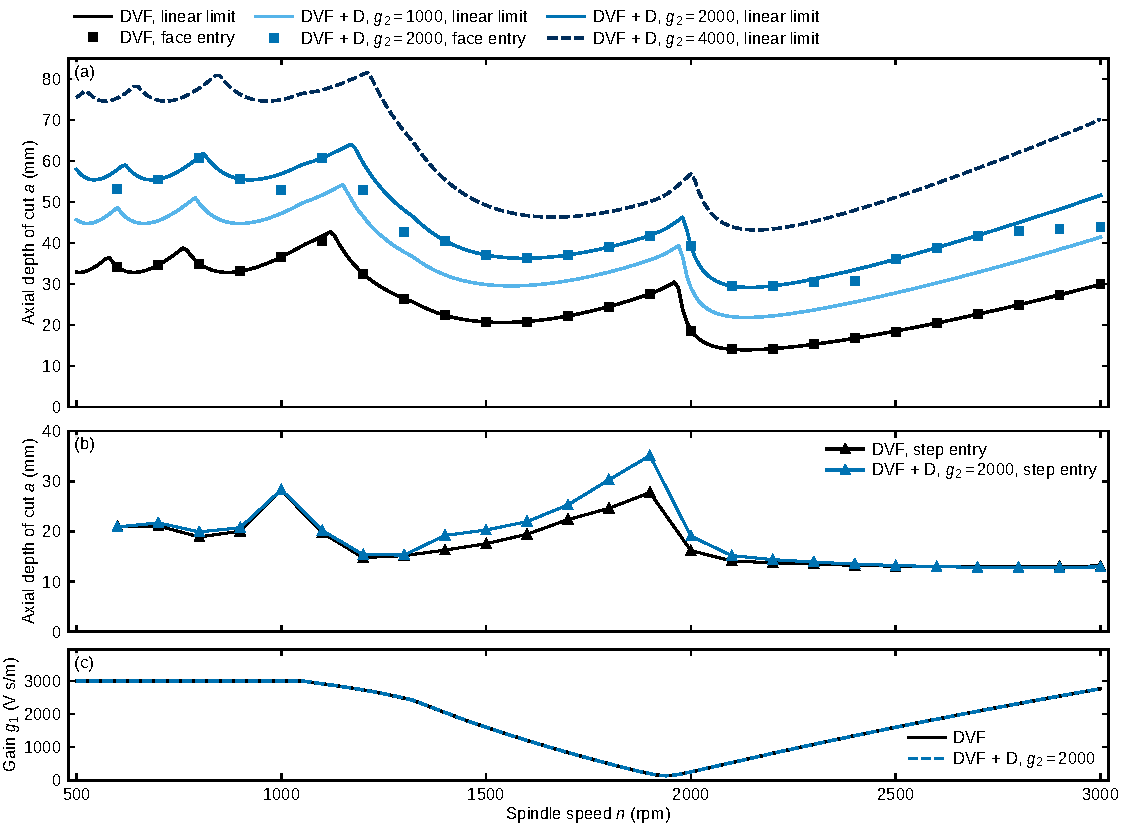
\includegraphics[width=\textwidth]{figures/fig08_delayed_limits.pdf}
  \caption{Designs obeying the same authority rule ($g_1\le\SI{3000}{\volt\second\per\metre}$; steady forced command within \SI{9}{\volt} up to 0.9 of the design's own $\alim$). (a)~Linear limits of DVF and of DVF\,+\,D with $g_2=1000$, 2000 and \SI{4000}{\volt\second\per\metre}; squares: simulated face-entry limits ($\lvert V\rvert\le\SI{9}{\volt}$, 25 speeds) of DVF and of DVF\,+\,D with $g_2=2000$. (b)~Simulated step-entry limits of the same two designs. (c)~Their admissible gain $g_1$.}
  \label{fig:dlim}
\end{figure}

\subsection{Entries in the simulator}\label{sec:delayed-entry}

Step and face entries (Section~\ref{sec:bistab-prot}) were simulated with the \SI{9}{\volt} clip at 25 speeds (\SIrange{600}{3000}{\rpm}) for DVF and for DVF\,+\,D with $g_2=2000$, with the depth ladder scaled to each design's own $\alim$ (Fig.~\ref{fig:dlim}a,b). The face-entry limit is 14.1--\SI{40.6}{\milli\metre} for DVF (at least $0.974\alim$) and 29.5--\SI{60.8}{\milli\metre} with D, 1.45--2.12 times higher (median 1.72); it reaches the new linear limit at 16 of the 25 speeds and stops at 0.85--$0.98\alim$ at the other nine. The step entry gains little: 12.9--\SI{28.2}{\milli\metre} for DVF against 12.7--\SI{35.1}{\milli\metre} with D, a ratio of 0.98--1.27 (median 1.03). From \SI{2100}{\rpm} upwards D adds at most \SI{1.1}{\milli\metre} and lowers the limit by up to \SI{0.2}{\milli\metre} at \SIrange{2700}{3000}{\rpm}: this limit is set by saturation during the entry, not by damping. Only between 1300 and \SI{2000}{\rpm}, where the step entry approaches the linear limit, does D raise it markedly, by up to 1.27 times (\SI{1900}{\rpm}). At \SIrange{600}{1300}{\rpm}, the larger DVF gain of this rule (2481--3000 instead of \SI{1500}{\volt\second\per\metre}) itself raises the step-entry limit 1.05--1.34 times above that of Section~\ref{sec:bistab-map} (cf.\ Section~\ref{sec:bistab-gain}).
% src: results/c4_entry.npz (designs feas_dvf, feas_d2000: a_entry, a_lim, g1; per-speed ratios; face entry with D below 0.98 a_lim at 600, 1000, 1200, 1300, 2300, 2400, 2800-3000 rpm), results/c4_summary.json (entry); results/c1_map.npz (a_step_clip at g = 1500 compared at the eight speeds 600-1300 rpm: ratios 1.05-1.34, recomputed; identical values at 1600-2400 rpm, where the gains coincide); README §13.6, §11.6

The range between the step-entry and the linear limit, in which the cut is bistable, therefore widens: the ratio of the two limits has a median of 0.704 for DVF and 0.390 with D, and the range a median width of 7.6 against \SI{25.9}{\milli\metre}. Most of the depth gained needs a gentle entry, and its basin is a few millimetres per second (Section~\ref{sec:delayed-valid}). The 300-revolution classifier biases these near-limit boundaries high (Section~\ref{sec:bistab-prot}); near the forced resonance (\SI{2000}{\rpm}), the face entry with the gain of Section~\ref{sec:feasibility} and $g_2=2000$ even reached the top of the depth ladder, $1.05\alim$, whereas runs of 2000 revolutions start to chatter at $0.9996\alim$.
% src: results/c4_entry.npz (step/a_lim medians 0.704 and 0.390; a_lim - step medians 7.56 and 25.88 mm); results/c4_summary.json (entry.edge_clip.paper+2000: max 1.05); verification/tdsim/check10_forced_resonance_long_runs.json (c4_face_entry: 2000 rpm, g1 = 250.9, g2 = 2000, td300 1.05, onset 0.9996); README §13.6

\subsection{Certified gain map}\label{sec:delayed-map}

The certified kick [Eq.~\eqref{eq:lmi-size} with $e=e_2$] was computed at the four speeds of Section~\ref{sec:bistab-basin} and 17 depths (2--\SI{34}{\milli\metre}) for 20 delayed pairs, $g_1\in\{500,1000,1500,2000,3000\}$ and $g_2\in\{500,1000,2000,4000\}$\,\si{\volt\second\per\metre}, and for DVF at 26 gains (500--\SI{3000}{\volt\second\per\metre} in steps of 100), so that DVF has no fewer candidates. The solver used its default settings, as for the surface of Section~\ref{sec:cert-c2}, and the certificates are corrected for the command bound as in Section~\ref{sec:cert-lmi} (factors 0.59--1, below 0.99 only where $u_0$ almost vanishes). Table~\ref{tab:dgap} gives the depth up to which every grid depth is certified with a kick of at least $\beta_{\mathrm{th}}$. At $\beta_{\mathrm{th}}=\SI{1}{\milli\metre\per\second}$ the delayed term covers the whole grid at all four speeds (28--\SI{34}{\milli\metre} with $g_2\le2000$), against 16--\SI{34}{\milli\metre} for DVF, and the advantage narrows as $\beta_{\mathrm{th}}$ grows. The threshold matters: a kick of \SI{1}{\milli\metre\per\second} carries only 0.5--\SI{1.3}{\percent} of the cutting impulse of one tooth period [Eq.~\eqref{eq:impulse}] at \SI{16}{\milli\metre} (0.2--\SI{0.6}{\percent} at \SI{34}{\milli\metre}), whereas kicks of 2.4--\SI{10.8}{\percent} tip the clipped DVF cut into chatter near its limit (Section~\ref{sec:bistab-basin}).
% src: src/c4_comb.py (GM_RPM, GM_DEPTH, GM_G1, GM_G2, GM_G1_DVF; run_gainmap, FAST settings); results/c4_gainmap.npz (delayed: 913 of 1360 certified, 270 unstable, 169 orbit saturates, 8 without a passing candidate; DVF: 835 of 1768, 722, 207, 4); results/c4_summary.json (gainmap.by_rpm.certified_without_gap_mm); results/c3_summary.json (errata.c4_gainmap: size_factor 0.593-1, table unchanged); paper/figures/figure_numbers.json (fig09.gainmap_factor); impulse shares recomputed from Eq. (impulse) with src/params.py: 0.48-1.25 % at 16 mm, 0.22-0.59 % at 34 mm; README §13.7, §14.9

Both families follow one pattern (Fig.~\ref{fig:dbasin}). The certificate-optimal DVF gain rises with the depth from 500 to 2200--\SI{2700}{\volt\second\per\metre}: the certificate picks the smallest gain with enough linear margin, itself an allocation of authority. With D, $g_1$ stays at 500--1000 while $g_2$ rises to 2000--4000 beyond the depths at which DVF loses its certificate, except at 24--\SI{26}{\milli\metre}, about twice the axial pitch, where the forced command is small, DVF is certified again and $g_1=1500$--2000 with $g_2=500$--1000 is chosen. Where both families are certified, the best delayed certificate exceeds the best DVF one by a median factor of only 1.05--1.08 per speed; the basin itself is measured next.
% src: results/c4_gainmap.npz (maximising designs per speed and depth; DVF optimum b_max 2.5-3.8 V at 24-26 mm); results/c4_summary.json (gainmap.by_rpm.comb_over_dvf medians 1.08, 1.05, 1.07, 1.06); README §13.7

\begin{table}[!tbp]
  \centering
  \caption{Certified depth without a gap (\si{\milli\metre}): the largest depth of the grid (2--\SI{34}{\milli\metre}, step \SI{2}{\milli\metre}) up to which every grid depth is certified with a kick of at least $\beta_{\mathrm{th}}$ by the best candidate design ($\lvert V\rvert\le\SI{9}{\volt}$; averaged collocation model; command bound corrected). $\ge34$: the whole grid.}
  \label{tab:dgap}
  \small
  \begin{tabular}{@{}llcccc@{}}
    \toprule
    $\beta_{\mathrm{th}}$ (\si{\milli\metre\per\second}) & Candidates & \SI{1090}{\rpm} & \SI{1420}{\rpm} & \SI{2500}{\rpm} & \SI{2870}{\rpm}\\
    \midrule
    1 & DVF, 26 gains & $\ge34$ & 18 & 16 & 28\\
      & DVF\,+\,D, 20 pairs & $\ge34$ & $\ge34$ & $\ge34$ & $\ge34$\\
      & DVF\,+\,D, $g_2\le2000$ & $\ge34$ & 30 & 28 & $\ge34$\\
    2 & DVF, 26 gains & 32 & 16 & 16 & 16\\
      & DVF\,+\,D, 20 pairs & $\ge34$ & 30 & 28 & $\ge34$\\
    4 & DVF, 26 gains & 26 & 16 & 14 & 14\\
      & DVF\,+\,D, 20 pairs & 28 & 26 & 16 & 18\\
    \bottomrule
  \end{tabular}
\end{table}
% src: results/c4_summary.json (gainmap.by_rpm.certified_without_gap_mm: dvf_*, comb_*, comb_g2le2000_1); results/c3_summary.json (errata.c4_gainmap.certified_without_gap_mm: unchanged by the correction); README §13.7 (table), §14.9

\subsection{Validation in the simulator}\label{sec:delayed-valid}

At the four speeds and 6--\SI{34}{\milli\metre}, 100 design points were simulated: the best DVF of the five-gain and of the 26-gain grid (22 and 21 points), the delayed design of the map (24 points up to \SI{26}{\milli\metre} and 8 at 30 and \SI{34}{\milli\metre}), and the \emph{same-$g_1$ design} (25 points), i.e.\ the $g_1$ of the 26-gain DVF optimum with the $g_2$ that maximises its certificate. The same-$g_1$ design has the forced orbit and the authority budget of that DVF, so any change of its basin is due to the delayed term alone. For each point the simulated critical kick $\Delta v^*$ (worst of 16 phases), the certificate with strict solver settings and its sampled check, and the critical kick of the averaged collocated model (\ref{app:lmi}) were computed; the 32 map designs also received the off-axis test of Section~\ref{sec:cert-c2}.
% src: src/c4_comb.py (VAL_DEPTH, VAL2_DEEP, best_gains, _same_g1, run_validate, run_validate2); results/c4_validate.npz (22 dvf, 24 comb), results/c4_validate2.npz (21 dvf_fine, 25 same_g1, 8 comb); README §13.8

No unkicked cut chattered. The certificate lies below $\Delta v^*$ at all 89 points where a kick of up to \SI{3}{\metre\per\second} ended in chatter (the other 11 lie at 6 and \SI{10}{\milli\metre} at \SI{1420}{\rpm} and at \SI{6}{\milli\metre} at \SI{2870}{\rpm}), by factors of 1.60--7.32 (median 2.29), and of 2.08--3.69 at the eight deepest points, with $g_2$ up to 4000. It lies below the critical kick of the averaged model at all 97 points where that kick is finite; none of the 2304 off-axis runs chattered; and the sampled check stayed at $\mathcal V\le0.998$, which is only a consistency check (Section~\ref{sec:cert-c2}). Despite the model error in the delayed velocity, no simulated point fell below its certificate.
% src: results/c4_validate.npz, results/c4_validate2.npz (unsettled 0; td_min infinite at 11 points; model_kick infinite at 3; offaxis 0/1728 and 0/576; proof_vmax 0.998); results/c4_summary.json (validate2: all_cert_below_td 89/89, all_cert_below_model 97/97); results/c3_summary.json (errata.c4_validate: corrected 1.60-7.32, median 2.29; deep 2.08-3.69); README §13.8, §14.9

Whether the basin itself widens was judged from $\Delta v^*$ at the 22 depth--speed pairs where both families have a finite value (Fig.~\ref{fig:dbasin}). The map design exceeds the 26-gain DVF by a median factor of 1.11 (0.82--3.02; larger at 18 of 22). Both DVF designs, however, are certificate optima rather than the widest simulated basins; against the better of the two the median ratio is 1.04 (0.81--3.02; ahead at 13 of 22), and 1.19 (0.99--3.02) at depths of \SI{18}{\milli\metre} and more. The same-$g_1$ design exceeds its DVF by a median factor of 1.14 (0.96--2.59; at 19 of 22).
% src: results/c4_summary.json (validate2: comb_over_dvf 0.82-3.02, median 1.11, 18/22; comb_over_better_dvf 0.81-3.02, median 1.04, 13/22; same_g1_over_dvf 0.96-2.59, median 1.14, 19/22; pairs_mmps); against the better DVF at >= 18 mm: 0.99-3.02, median 1.19, recomputed from pairs_mmps; README §13.8

Where the DVF certificate almost vanishes, the basin widens with the same budget. A rule fixed before the simulations were compared, a DVF certified kick of at most \SI{2.1}{\milli\metre\per\second}, selects six pairs at 18--\SI{34}{\milli\metre}, at which the same-$g_1$ design raises $\Delta v^*$ 1.79--2.59 times (median 2.00), e.g.\ from 4.0 to \SI{10.4}{\milli\metre\per\second} at \SI{1420}{\rpm} and \SI{18}{\milli\metre}; the next pair, with a DVF certificate of \SI{2.6}{\milli\metre\per\second}, gives 1.45, and the 13 pairs at \SI{18}{\milli\metre} and deeper give 1.06--2.59 (median 1.45). In every same-$g_1$ design the certificate chose $g_2=500$, the smallest of the grid, and no other $g_2$ was simulated: this is a choice, not a tested optimum. The delayed term thus widens the basin through its linear margin, not only by freeing authority; freeing authority can add to it (\SI{2500}{\rpm}, \SI{22}{\milli\metre}: the map design, $g_1=500$ with a forced command of \SI{2.5}{\volt} instead of \SI{7.7}{\volt}, reaches 7.8 against \SI{5.4}{\milli\metre\per\second}). Below \SI{18}{\milli\metre} the basin does not widen: the same-budget ratio is 0.96--1.16, and the map design can narrow it because the certificate prefers a smaller $g_1$ (\SI{1420}{\rpm}, \SI{14}{\milli\metre}: 17.9 against \SI{21.8}{\milli\metre\per\second}). The gains that maximise the certificate are not those that maximise the basin.
% src: results/c4_summary.json (validate2.same_g1_near_dvf_limit: rule DVF certified kick <= 2.1 mm/s, 6 pairs: 1420 rpm at 18 and 22 mm, 2500 rpm at 22 mm, 2870 rpm at 18 and 22 mm, 1090 rpm at 34 mm; 1.79-2.59, median 2.00; next pair 1090 rpm, 30 mm: 1.45; same_g1_deep: 13 pairs, 1.06-2.59, median 1.45; pairs_mmps: 1420 rpm, 18 mm: 4.02 -> 10.42 mm/s); results/c4_validate2.npz (same_g1: g2 = 500 at all 25 points); results/c4_gainmap.npz (2500 rpm, 22 mm: b_max 2.46 V at g1 = 500 and 7.68 V at g1 = 1900); README §13.8

\begin{figure}[!tbp]
  \centering
  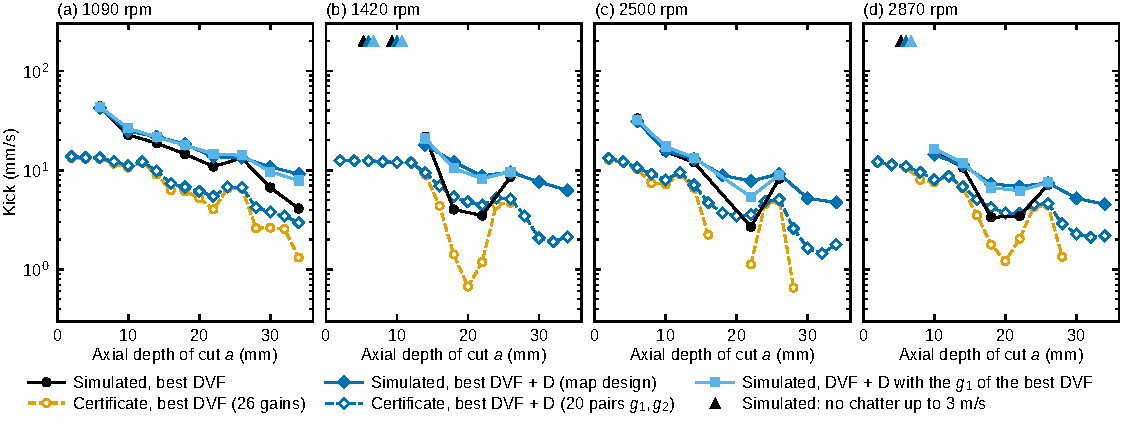
\includegraphics[width=\textwidth]{figures/fig09_delayed_basin.pdf}
  \caption{Certified and simulated kicks with the delayed term at (a)~1090, (b)~1420, (c)~2500 and (d)~\SI{2870}{\rpm} ($\lvert V\rvert\le\SI{9}{\volt}$). Open markers: certified kick of the best design at each depth over 26 DVF gains (circles) and over 20 delayed pairs $(g_1,g_2)$ (diamonds), command bound corrected; no marker: nothing certified. Filled markers: simulated critical kick $\Delta v^*$ (worst of 16 phases) of the best DVF design (26 gains), of the delayed design of the map, and of the same-$g_1$ design ($g_2=\SI{500}{\volt\second\per\metre}$ added to the $g_1$ of that DVF); triangles: no chatter for any kick up to \SI{3}{\metre\per\second}.}
  \label{fig:dbasin}
\end{figure}

\subsection{Robustness}\label{sec:delayed-robust}

The results above assume one mode, an instantaneous loop, a comb delay equal to $T$ and identical teeth. These assumptions were relaxed with Eq.~\eqref{eq:comb-char} at the four speeds (Table~\ref{tab:drobust}, Fig.~\ref{fig:robust}), for designs that keep \SI{10}{\percent} of the voltage free (forced command below \SI{8.1}{\volt} up to $0.9\alim$; $g_1=1396$--\SI{2539}{\volt\second\per\metre}): a design whose demand reaches exactly \SI{9}{\volt}, as in Sections~\ref{sec:feasibility}--\ref{sec:certificates}, saturates under any perturbation.
% src: src/c4_robust.py (GUARD = 0.9, designs, EPS, RUNOUT, TAU, MODE2, N_DEPTH = 40); results/c4_robust.npz (g1 1395.8-2539.5 V s/m, equal across g2 within 1.1 V s/m); README §13.9

\emph{Comb-delay error.} A speed error or a delay rounded to samples gives $T_c\neq T$, and the comb no longer vanishes on the orbit. For $g_2=2000$ and errors of $\pm\SI{2}{\percent}$ the limit changes by $+8$ to $+\SI{17}{\percent}$ ($-\SI{2}{\percent}$) and by $-7$ to $-\SI{13}{\percent}$ ($+\SI{2}{\percent}$), and the worst forced command, 7.8--\SI{8.9}{\volt}, stays within the margin (Fig.~\ref{fig:robust}a,d). At $+\SI{2}{\percent}$, however, the limit falls to 0.87--0.93 of its nominal value, into the design depths (up to $0.9\alim$) at three of the four speeds; at $\pm\SI{1}{\percent}$ it stays within 0.93--1.08. At $\pm\SI{3}{\percent}$ the forced command exceeds \SI{9}{\volt} in two of the eight cases. In the simulator, the face entry at \SI{2500}{\rpm} follows the shifted limit (from 36.2 to \SI{28.7}{\milli\metre} as the error goes from $-2$ to $+\SI{2}{\percent}$) within \SI{0.1}{\percent}.
% src: results/c4_robust.npz, results/c4_summary.json (robust.by_rpm, tooth comb: eps_a_lim_mm, eps_worst_cmd_V; td_face_eps: 28.74/28.77 to 36.22/36.25 mm); paper/figures/figure_numbers.json (fig10: eps_plus2_rel 0.87-0.93, eps_minus2_rel 1.08-1.17, eps_pm1_rel 0.93-1.08, eps_pm2_worst_cmd 7.76-8.89 V, eps_pm3_cases_above_9V 2 of 8: 2500 rpm at -3 %, 1420 rpm at +3 %); README §13.9

\emph{Runout.} Eccentric runout makes the forced orbit spindle-periodic, so the comb acts on it, as does the regeneration. The runout at which the worst forced command (40 depths up to $0.9\alim$, eight runout phases) reaches \SI{9}{\volt} falls as $g_2$ grows, except between DVF and $g_2=1000$ at \SI{2870}{\rpm}, from 1.12--\SI{4.50}{\micro\metre} for DVF to 0.69--\SI{1.73}{\micro\metre} for $g_2=4000$ (Table~\ref{tab:drobust}; Fig.~\ref{fig:robust}b,e).
% src: results/c4_summary.json (robust.by_rpm: runout_tolerance_um, DVF/1000/2000/4000 in um: 1090 rpm 3.63/3.22/2.42/1.73, 1420 rpm 4.50/1.98/1.75/1.27, 2500 rpm 1.55/1.50/1.33/0.84, 2870 rpm 1.12/1.22/1.03/0.69); src/c4_robust.py (worst_orbit_command: N_DEPTH = 40, n_psi = 8); README §13.9

\emph{Loop delay and unmodelled modes.} With the identified mode alone, DVF\,+\,D loses limit gradually with the loop delay and stays above DVF (\SI{400}{\micro\second}, $g_2=2000$: 24.0--35.8 against 17.3--\SI{31.7}{\milli\metre}). Higher modes, not identified for this set-up, were assumed: $k_2=6k$ at 400 and \SI{600}{\hertz}, $k_2=40k$ at \SI{800}{\hertz}, $\zeta_2=\SI{1}{\percent}$. With the \SI{400}{\hertz} mode and \SI{300}{\micro\second}, $g_2=2000$ falls below DVF at all four speeds (11.0--22.4 against 17.1--\SI{40.1}{\milli\metre}); with the \SI{600}{\hertz} mode and \SI{200}{\micro\second} it collapses to 4.4--\SI{12.9}{\milli\metre}, while $g_2=1000$ stays above DVF (23.7--\SI{46.8}{\milli\metre}; Fig.~\ref{fig:robust}c,f). DVF itself collapses at \SI{400}{\micro\second} with the 600 and \SI{800}{\hertz} modes. The cause is the phase of the comb, not its gain: at the collapse point (\SI{2500}{\rpm}, \SI{300}{\micro\second}, \SI{400}{\hertz}) the critical root lies near \SI{473}{\hertz}, where $\lvert K\rvert=\SI{2861}{\volt\second\per\metre}$ is about half its peak $g_1+2g_2=\SI{5396}{\volt\second\per\metre}$ but the phase of $K$ [Eq.~\eqref{eq:comb-K}], $-\ang{36}$, adds to the lag of the delay. DVF with the constant gain $g_1+2g_2$ keeps a limit more than three times larger under the same delay and mode.
% src: results/c4_summary.json (robust.by_rpm tau_a_lim_mm: one mode at 400 us 24.04-35.77 against 17.29-31.68 mm; mode_400Hz at 300 us 10.99-22.37 against 17.06-40.06 mm; mode_600Hz at 200 us 4.41-12.92 mm, g2 = 1000 23.74-46.84 mm; DVF at 400 us: 0 with 600 Hz, 0-1.83 mm with 800 Hz); README §13.9 (473 Hz, |K| = 2861 V s/m, -36 deg: README only; consistent with |K(i 2 pi f)| = 2898-2860 V s/m at -36.0 deg for f = 473.0-473.5 Hz, g1 = 1395.8); tests/test_c4_comb.py (test_comb_fragility_to_delay_is_its_phase_not_its_gain: limit with g1 + 2 g2 more than 3 times that of the comb)

\emph{Spindle-period comb.} With $T_c=N_tT$ the comb vanishes on the runout and tolerates it like DVF (1.12--\SI{4.46}{\micro\metre}), but it is no remedy: without delay its limit is close to that of DVF ($+0.3$ to $+\SI{4}{\percent}$; $+\SI{27}{\percent}$ at \SI{2500}{\rpm}), and it is very sensitive to phase (at \SI{2500}{\rpm} the limit jumps from 20 to \SI{80}{\milli\metre} with \SI{100}{\micro\second} of delay) and to speed errors (9.7--\SI{13.6}{\volt} of forced command at $-\SI{2}{\percent}$).
% src: results/c4_summary.json (robust.by_rpm spindle comb: a_lim 39.18/20.08/20.16/22.89 mm against DVF 37.64/19.40/15.91/22.82 mm; runout_tolerance_um 1.12-4.46; 2500 rpm, one mode: 20.16 -> 80.24 mm at 100 us; eps_worst_cmd_V 13.62 V at -2 %); README §13.9

\begin{table}[!tbp]
  \centering
  \caption{Robustness at 1090, 1420, 2500 and \SI{2870}{\rpm} (ranges over the speeds; closed-form zero-order model; forced command below \SI{8.1}{\volt} up to $0.9\alim$). Runout: eccentric runout at which the largest forced command over the design depths and eight runout phases reaches \SI{9}{\volt}. Loop delay: largest of the computed delays (0, 50, 100, 200, 300, \SI{400}{\micro\second}) with $\alim(\tau)\ge0.5\,\alim(0)$ at every speed and for each assumed second mode (400, 600 or \SI{800}{\hertz}).}
  \label{tab:drobust}
  \small
  \begin{tabular}{@{}lcccc@{}}
    \toprule
     & DVF & \multicolumn{3}{c}{DVF\,+\,D, $g_2$ (\si{\volt\second\per\metre})}\\
    \cmidrule(l){3-5}
     & & 1000 & 2000 & 4000\\
    \midrule
    Linear limit (\si{\milli\metre}) & 15.9--37.6 & 24.6--47.1 & 32.1--55.4 & 45.8--70.5\\
    Runout tolerated (\si{\micro\metre}) & 1.12--4.50 & 1.22--3.22 & 1.03--2.42 & 0.69--1.73\\
    Loop delay tolerated (\si{\micro\second}) & 300 & 200 & 100 & 100\\
    \bottomrule
  \end{tabular}
\end{table}
% src: results/c4_summary.json (robust.by_rpm: a_lim_mm, runout_tolerance_um, tau_a_lim_mm); paper/figures/figure_numbers.json (fig10: runout_tolerated_um, loop_delay_largest_with_ratio_ge_05_us); README §13.9 (table)

\begin{figure}[!tbp]
  \centering
  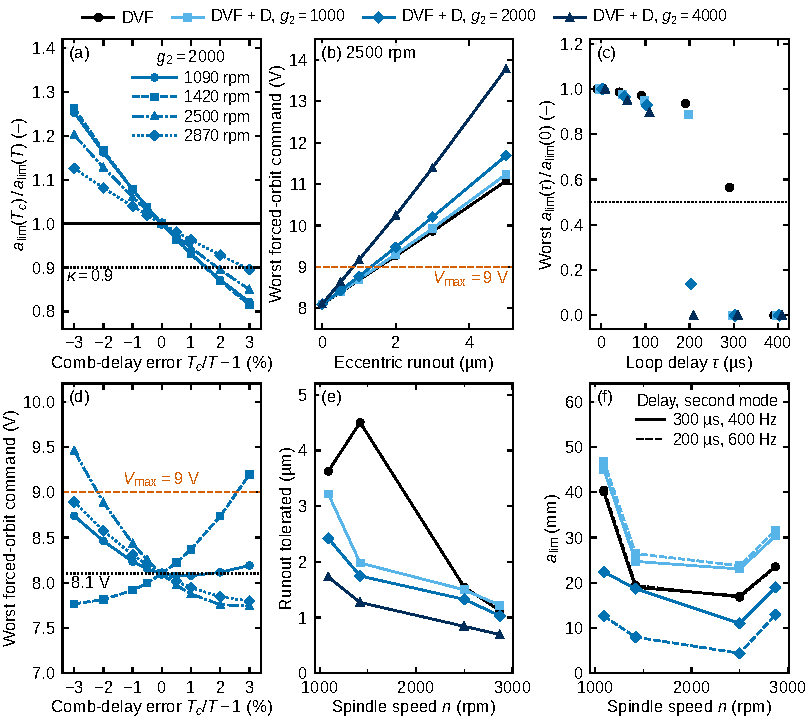
\includegraphics[width=\textwidth]{figures/fig10_robustness.pdf}
  \caption{Robustness of the delayed term (closed-form zero-order model; designs as in Table~\ref{tab:drobust}). (a)~Linear limit against the comb-delay error, relative to the exact delay ($g_2=\SI{2000}{\volt\second\per\metre}$), and (d)~worst forced-orbit command in the same cases. (b)~Worst forced-orbit command at \SI{2500}{\rpm} against the eccentric runout, and (e)~the runout at which it reaches \SI{9}{\volt}. (c)~$\alim(\tau)/\alim(0)$, worst over the four speeds and the three assumed second modes, at the computed delays only (0: loop unstable without cutting). (f)~$\alim$ with \SI{300}{\micro\second} and the \SI{400}{\hertz} mode (solid) or \SI{200}{\micro\second} and the \SI{600}{\hertz} mode (dashed); $g_2=4000$, unstable without cutting in both cases, is not shown.}
  \label{fig:robust}
\end{figure}

\subsection{Implications and limitations}\label{sec:delayed-lim}

The delayed term thus buys linear margin, and basin where DVF is weakest, at a cost in robustness that grows with $g_2$. A gain $g_2\approx\SI{1000}{\volt\second\per\metre}$ keeps 1.23--1.57 times the DVF limit (Table~\ref{tab:dlim}) and tolerates \SI{200}{\micro\second} with the assumed modes, whereas 2000--\SI{4000}{\volt\second\per\metre} need a loop of \SI{100}{\micro\second} or less. An implementation would need a fast loop, a multi-mode frequency response in the design, phase compensation of the D branch (not tested here), a delay synchronised with the spindle encoder, runout of about 1--\SI{2}{\micro\metre} or less, and an authority margin: \SI{10}{\percent} of the voltage covers speed errors of $\pm\SI{2}{\percent}$ up to $g_2=2000$ (at 4000 the forced command exceeds \SI{9}{\volt} in three of the eight cases) and runout of 1.0--\SI{2.4}{\micro\metre} at $g_2=2000$, but a \SI{10}{\percent} depth margin covers speed errors of only about $\pm\SI{1}{\percent}$ at $g_2=2000$.
% src: results/c4_summary.json (limits.feasible.d1000.ratio_to_dvf 1.23-1.57; robust.by_rpm: tooth comb 4000 eps_worst_cmd_V above 9 V in 3 of the 8 cases at +-2 %; tooth comb runout_tolerance_um 1.03-2.42); README §13.10

Four limitations add to those of Sections~\ref{sec:bistability} and~\ref{sec:certificates}. Only one mode was identified; the second modes are assumed. The certificate holds for the $N$-node collocation of the averaged model, not for the delay equation, and its delayed velocity departs from that of the delay equation after a kick. The robustness results come from the closed-form zero-order model, checked against the simulator except for the second modes, with runout in the regenerated chip only. Measurement noise and the stroke of the actuator are not modelled. Nothing was tested experimentally.
% src: README §13.10 (limits)
